\documentclass[main.tex]{subfiles}
\begin{document}

\section{’t Hooft-Polyakov Monopoles}
In this section, it will be shown that free magnetic monopoles in the physical vacuum are possible as regular solutions of the field equations of the Georgi-Glashow model, following the notorious works published by Gerard 't Hoft \cite{Hof:Mon} and Aleksander Polyakov \cite{Pol:Mon} in 1974. 
\subsection{An Intuitive Example}
A simple and very clarifying example, taken from \cite{Hof:Mon}, will be discussed in order to give an intuitve idea of how it is possible to have monopoles in quantum field theory.  \\
We should consider a two-dimensional spherical surface $S^2$ in the usual 3D space, with some magnetic flux $\Phi$ entering only in a spot. If the spot is surrounded by a contour $C_0$ along which the fields are null, the potential around $C_0$ should be equal to: 
\begin{equation}
    A_i = \partial_i \Lambda 
\end{equation}
\begin{figure}[hb]
\centering
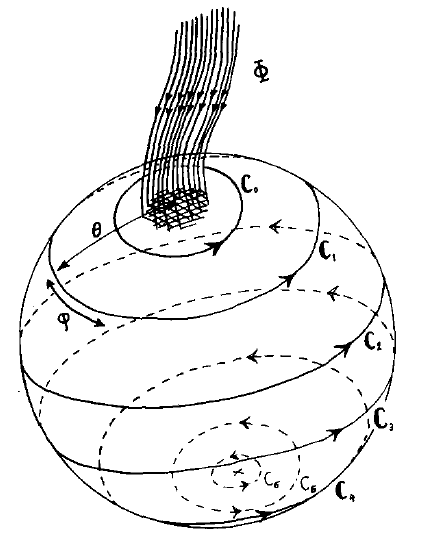
\includegraphics[scale=0.35]{thooft.png}
\caption{'t Hooft schematization of the spherical surface and the spot}
\label{fig-THooft}
\end{figure}
where $\Lambda$ is a gauge transformation, which acts on the wavefunction in this way: $\psi \rightarrow e^{i\Lambda} \psi $. 
While $\Lambda$ is multivalued, $\Phi$, being a physical field, is required to be a single-valued function. Since, 
\begin{equation}
    \Phi = \int_{C_0} \partial_i \Lambda \dd{l}^i,
\end{equation} 
$\Phi$ should be equal to an integer multiplied by $2 \pi  $, a complete gauge rotation along the contour. 
In an Abelian gauge theory, there must be another spot from which the flux comes out, because the $2k \pi$ rotation cannot be continuously changed into a constant lowering the contour $C_0$ over the sphere. \\ 
Instead, in a non Abelian gauge theory, with a compact covering group, such as O(3), a $2k\pi$ rotation with even $k$ can be shifted into a constant without singularity.
This implies that if we have a non Abelian gauge theory with a compact covering group and such compact covering group has the electromagnetic group U(1) as a subgroup, the existence of the magnetic monopole would be allowed without supposing the existence of any singularity anywhere on the sphere.
A theory that satisifies those requirements is the Georgi-Glashow model for the electroweak interaction.

\subsection{The bosonic part of the Georgi-Glashow Model}
The Georgi-Glashow model was proposed as a theory for the electroweak interaction and, in its bosonic part, is based on the gauge group SU(2) which two-to-one homomorphic to SO(3).\\
The lagrangian density $\mathcal{L}$, whose associated action is invariant under gauge transformation belonging to SO(3), contains the Higgs field $\vec{\phi} = ( \phi^1, \phi^2 , \phi^3)$, which is a vector in the adjoint representation of SO(3) and three gauge potentials $\Vec{W}^\mu$, with values in the Lie algebra of SO(3). 
We use superscript arrows to denote objects which take values in the adjoint representation of SO(3).
$\mathcal{L}$ has the following form: 
\begin{equation}
\mathcal{L}= \frac{1}{2}D_{\mu}\phi^a D^\mu \phi^a  -\frac{1}{4} G_{\mu \nu}^a G^{a \ \mu \nu} - \underbrace{\frac{1}{4}\lambda (\phi^2 -a^2)}_{V(\phi)},
\label{eq:lag}
\end{equation}
where $\Vec{G_{\mu \nu}}$ is the gauge field-strength, defined as follows:
\begin{equation}
\Vec{G_{\mu \nu}} = \partial_{\mu}  \Vec{W}^\nu -\partial_{\nu}  \Vec{W}^\mu - e \Vec{W}^\nu \times \Vec{W}^\mu,
\end{equation}
and the operator $D_{\mu}$ is the gauge covariant derivative: 
\begin{equation}
D_\mu \Vec{\phi} = \partial_\mu \Vec{\phi} - e \Vec{W}_\mu \times \Vec{\phi}.
\end{equation}
Let us look at the physical meaning of each term in the lagrangian density:
\begin{itemize}
    \item The term $\frac{1}{2}D_{\mu}\phi^a D^\mu \phi^a $ is the free field term;
    \item The term  $-\frac{1}{4} G_{\mu \nu}^a G^{a \ \mu \nu}$ describes the dynamics of the potential $\Vec{W}_{\mu}$;
    \item The term  $V(\phi) $ describes the self interaction of the Higgs field and contains a non negative constant $\lambda$.
\end{itemize}

\paragraph{Spectrum of the Model}
Now we are interested in the spectrum of the model. It can be obtained through perturbation theory, considering a Higgs potential with little fluctuation around the minimum $\vec{a}$:
\begin{equation}
\vec{\phi} = \vec{a}+ \vec{\chi}. 
\end{equation} 
Four bosons figure in our model: the photon $A_{\mu} = \frac{1}{a} \vec{a}\cdot \vec{W}_\mu $, the Higgs Boson, associated to the field $\vec{\phi}$ and the bosons $\vec{W}_\mu^\pm$. Their properties are shown in table \ref{tab:Bosons}.
\begin{table}[H]
\centering
\begin{tabular}{cc|cc}
\toprule
 Field  &   Definition   &  Mass  &  Charge \\
 \midrule
 $A_{\mu}$ &          Photon                   &  0                             &     0 \\
 $\phi $   &          Higgs Boson              &  $a \sqrt{2 \lambda} \hbar $   &     0 \\
$ W_{\mu}^{\pm} $&    Two Massive Bosons &  $ae\hbar$                     &    $ \pm e \hbar$ \\
 \bottomrule
\end{tabular}
\caption{Bosonic Spectrum of the Georgi-Glashow model.}
\label{tab:Bosons}
\end{table}
%
%
For the sake of simplicity, we choose as a minimum the vector $\vec{a}= (0,0,a)$. Then, working in the so-called unitary gauge, the fluctuation vector $\vec{\chi}$ can be written in such a way that $\vec{\chi} = (0,0,\chi) $.
At this point, we should expand the Higgs field around $\vec{a}$ in order to read the masses of the bosons from the quadratic term coefficients:
\begin{subequations}
 \begin{gather}
V(\phi)\simeq  \frac{1}{2}  \left(\sqrt{2 \lambda} a\right)^2 \chi^2 = \left( \frac{M_\chi}{\hbar }\right)^2 \chi^2 \\
 \frac{1}{2}D_{\mu}\vec{\phi} \cdot  D^\mu \vec{\phi} \simeq  \frac{1}{2}D_{\mu}\vec{a} \cdot  D^\mu \vec{a}  + \frac{1}{2} \left( ea \right)^2 =\frac{1}{2}D_{\mu}\vec{a} \cdot  D^\mu \vec{a}  + \frac{1}{2} \left( \frac{M_W}{\hbar} \right)^2
\end{gather}
\end{subequations}


To deduce the charges of the bosons, instead, we should see how the covariant derivative, which describese the minimal coupling for the photon $A_{\mu}$: 
\begin{equation}
\nabla_\mu = \partial_\mu + i \frac{Q}{\hbar} A_{\mu}
\end{equation}
is embedded in the SO(3) covariant derivative. Then, the value given to $Q$ for each boson, represents the charge of the bosons. 

\paragraph{Vacuum Configurations}Another aspect of the Georgi-Glashow model, which is relevant for understanding the 't Hooft-Polyakov monopoles, is the study of the vacuum configurations.\\
Using Noether's theorem, the stress energy tensor can be calculated. To be more specific, we are interested in its component $T^{00}$, which describes the energy density: 
\begin{equation}
T^{00} = \frac{1}{2} \Vec{E}^i \cdot  \Vec{E}^i + \frac{1}{2} \Vec{B}^i \cdot \Vec{B}^i +\frac{1}{2} D_0 \Vec{\phi} \cdot D_0 \Vec{\phi} +\frac{1}{2} D_i \Vec{\phi} \cdot  D_i \Vec{\phi} + V(\phi),
\label{eq:Den}
\end{equation}
where $\Vec{E}^i = - \Vec{G}^{0i}$  and $\Vec{B}^i$ is defined through this relation: $ \Vec{G}_{ij} = \epsilon_{ijk} \Vec{B}_k$.\\
Imposing that the energy density $T_{00}$, contained in expression \ref{eq:Den}, is null, we get the conditions for the vacuum configurations: 
\begin{equation}
\Vec{G}_{\mu \nu} = 0 \qquad D^{\mu} \Vec{\phi}  = 0 \qquad V(\phi)=0
\end{equation}
The last two of those conditions give the so-called \textit{Higgs Vacuum} configurations. 
In the Higgs vacuum, the Higgs field is such that $\vec{\phi}^2 = \vec{a}^2$. It follows that such vacuum configurations are not invariant under the whole SO(3) but under the subgroup SO(2)$\simeq$U(1), which is the gauge group of electromagnetism. Hence, the Georgi-Glashow model undergoes a spontaneous symmetry breaking process.

\subsection{The 't Hooft-Polyakov Ansatz}
\label{sect:Ansatz}
 \paragraph{Hypotheses}We are now interested at solutions of the Euler-Lagrange equations of the Georgi-Glashow model, characterised by the following properties: 
 \begin{enumerate}
     \item Finite Energy; 
     \item Stability; 
     \item Spherical Symmetry;
     \item Static Nature.
 \end{enumerate}
 
 In order to satisfy the first condition, we require that the following integral has a finite value: 
 \begin{equation}
 E = \int_{\mathbb{R}^3} T_{00} \dd[3]{x}.
 \end{equation}
 This is equivalent to asking that at spatial infinity the Higgs Field $\vec{\phi}$ approaches the Higgs Vacuum, which is represented by the set $\mathcal{M}_0 = \{ \vec{\phi}(\vec{r})  \mid  \vec{\phi}^2 = \vec{a}^2 \}$. 
 Hence, denoting as $\Sigma_{\infty}$ the spherical surface in $\mathbb{R}^3$ with an infinite radius, we require the existence of a continuous function, 
 \begin{equation}
     \phi_{\infty} \colon \Sigma_{\infty}  \to \mathcal{M}_0 ,
  \end{equation}
 such that:
 \begin{equation}
     \lim_{|\vec{r}|\to \infty} \vec{\phi}(|\vec{r}| \ \hat{r}) = \vec{\phi}_{\infty}(\hat{r}).
 \end{equation}
  Those functions belong to the second homotopy group $\Pi_2(\mathbb{R}^3)$ and can be classified according to their \textit{winding number}, which is a topological invariant and specifies the number of times the map wraps around $\mathcal{M}_0$.
  \medskip
  
  The second condition can be read as the request for non-dissipative solutions, that will never evolve in time to a configuration where $\vec{\phi}_{\infty}$ is constant. In mathematical terms, we are asking for the \textit{winding number} of the map $\vec{\phi}_{\infty}$ to be different from 0.
  \medskip
  
  The third and fourth conditions are imposed in order to simplify the problem: we will discuss a more general result, obtained without them, in section \ref{sect:top}.
  By static nature of the solutions, we mean that that the fields have to be time-indipendent and that $\vec{W}^{\mu = 0}= 0$ at any time. The latter is more than a simple gauge-fixing, because we require the time component of the gauge field to be null \textit{at any time}, which equates to saying that the gauge-fixing transformation, which brings us to $ \vec{W}^{\mu = 0}= 0$, has to be time-indipendent. Taking the expression \ref{eq:Den} for the energy density and imposing the static nature condition, we get that: 
  \begin{equation}
      E = \int_{\mathbb{R}^3} T_{00} = - \int_{\mathbb{R}^3} \mathcal{L} = -L
      \label{eq:En}
  \end{equation}
 
   \paragraph{Serach for the solutions}The spherical symmetry condition, instead, allows us to claim that there might exist two real functions of the paramer $\xi \equiv aer$, where $a$ is the module of the Higgs minimum $\vec{a}$ and $e$ is the electric charge: $H(\xi)$ and $K(\xi)$. We rescale the radial variable with $\xi$ for convenience in our future calculations. Hence, the ansatz for the solution to the Euler-Lagrange equations of the Georgi-Glashow model, might have this form: 
\begin{subequations}
  \begin{align}
      \vec{\phi}(\vec{r}) &= \frac{\vec{r}}{er^2}H(\xi) \\ 
      W^{\mu =i}_{a} &= - \epsilon_{aij}\frac{r^j}{er^2}(1 - K(\xi)) \\
      W^{\mu=0}_{a}&=0. 
  \end{align}
\end{subequations}
  
  Plugging these fields into the Euler-Lagrange equations of the model, we obtain two differential equations describing the dynamics of $H(\xi)$ and $K(\xi)$: 
  \begin{subequations}
  \begin{align}
  \xi ^2 \dv[2]{K}{\xi} &= KH^2 + K(K^2-1)   \label{eq:H}\\
  \xi ^2 \dv[2]{H}{\xi} &= 2K^2H + \frac{\lambda}{e^2}H (H^2 -\xi^2), \label{eq:K}
  \end{align}
  \end{subequations}
  
  In order to find the boundary conditions for the differential equations above, we should write the energy of the system as a function of $H(\xi)$ and $K(\xi)$:

  \begin{equation}
  \begin{split}
  E = \frac{4 \pi a}{e} \int_{0}^{\infty} \frac{\dd{\xi}}{\xi^2}  \bigr( \xi^2\dv{H}{\xi}  &+  \frac{1}{2}\left( \xi \dv{H}{\xi} -H \right)^2  +  
  \frac{1}{2} \left( K^2 - 1 \right)^2 +  \\
  & +K^2 H^2 + \frac{\lambda}{4e^2} \left( H^2-\xi^2\right)^2   \bigr)
  \end{split}
  \end{equation}
and require that such an integral has a finite value. It follows that: 
\begin{subequations}
  \begin{align}
 && \xi \to \infty &\colon  \quad \frac{H}{\xi} \to 1 \qquad \ K \to 0     \label{eq:bound1}\\
 && \xi  \to 0      &\colon  \quad H \sim  O(\xi)     \quad K \sim \ 1 + O(\xi)  \label{eq:bound2}
  \end{align}
\end{subequations}
 
 We should note that the condition that $H(\xi)$ approaches  spatial infinity linearly in $\xi$ implies that asymptotically the Higgs field has the following form: 
 \begin{equation}
 \vec{\phi}_{\infty}(\vec{\hat{r}}) = \lim_{|\vec{r}| \to \infty } \frac{\vec{r}}{er^2}H(aer) = a \hat{r}.
 \end{equation}
 This means that $\vec{\phi}_{\infty}$ is homotopic to the identity and has a winding number equal to 1. Therefore, those boundary conditions also ensure the non-dissipative nature of the  't Hooft-Polyakov solution.
 
Another aspect that deserves to be discussed is the existence of a solution for the system of equations \ref{eq:H} and \ref{eq:K}, given the boundary conditions \ref{eq:bound1} and \ref{eq:bound2}. It has been proved that a solution actually exists \cite{Taubes:Sol}.

\paragraph{Asymptotic form for the 't Hooft-Polyakov Solutions} 
We wish now to study the behaviour of the solutions of equation \ref{eq:H} and \ref{eq:K} in the limits for $r \to 0$ and $r \to \infty$ and then finally show that they describe an object of finite size that at big distances behaves analogously to the Dirac Monopole.\\

In the $r \to 0$ limit, we observe that the solutions for the fields, given the boundary conditions \ref{eq:bound1} and \ref{eq:bound2}, show no singularity: 
\begin{equation}
  \begin{cases}  
  H \sim \xi^2\\
  K \sim 1 + C \xi^2 
  \end{cases}
  \implies
  \begin{cases}
  \vec{\phi} \sim \vec{r}\\
  W^{i}_{a} \sim \epsilon_{aij}x^j
  
  \end{cases}
\end{equation}
This implies that also   $\vec{G}_{\mu \nu}$ is smooth and regular in the origin. Such evidence is a relevant difference, between the Dirac Monopole where the fields show a singularity in the origin, and the 't Hooft-Polyakov Monopole where no singularity in the origin occurs. \\

In the limit $r \to \infty$, equations \ref{eq:H} and \ref{eq:K}, provided the boundary conditions \ref{eq:bound1} and \ref{eq:bound2}, have such form: 
\begin{equation}
\begin{cases}
\dv[2]{K}{\xi}    = K    \\
\dv[2]{h}{\xi}   =  \frac{2 \lambda}{e^2} h \\
\end{cases}
\implies
\begin{cases}
K \sim e^{-\xi} = e^{- \frac{M_W r}{\hbar}}\\
h \sim e^{-\xi \sqrt{\frac{2 \lambda}{e^2}}} = e^{- \frac{M_H r}{\hbar}} \\
\end{cases}
\end{equation}
where $h:= H - \xi$.
Hence, the object we are looking at has finite dimensions, comparable with the Compton wave lengths $\frac{\hbar}{M_H}$ and $\frac{\hbar}{M_W}$. \\

In order to prove that such an object at spatial infinity behaves like a monopole, we should look at the electromagnetic field, which, in the Georgi-Glashow model is described by the following expression: 
\begin{equation}
 F_{\mu \nu} = \frac{1}{a} \vec{\phi} \cdot \vec{G}_{\mu \nu },
\end{equation}
and in the limit $r \to \infty$  gives:
\begin{equation}
F_{0i}= 0 \qquad F_{ij}= \epsilon_{ijk} \frac{r^k}{e r^3}.
\end{equation}
Hence, the asymptotic magnetic and electric fields are: 
\begin{equation}
\vec{E}=0 \qquad  \vec{B}= - \frac{1}{e} \frac{\vec{r}}{r^3}\,;
\end{equation}
they are compatible with a magnetic charge of: 
\begin{equation}
m= \frac{-4 \pi}{e},
\end{equation}
which is admitted by the Dirac quantization condition.

\todo{
Discutere un possibile commento sul fatto che tale carica sia la minima possibile
}
%%%%%%%%%%%%%%%%%%%%%%%%%%%%%%%%%%%%%%%%%%%%%%%%%%%%%%%%%%%%%%%%%%%%%%%%%%%%
\subsection{Extension to non-static and time-dependent solutions}
%%%%%%%%%%%%%%%%%%%%%%%%%%%%%%%%%%%%%%%%%%%%%%%%%%%%%%%%%%%%%%%%%%%%%%%%%%%%%%%
\label{sect:top}
In this section we will try to extend the 't Hooft-Polyakov ansatz to generic finite-energy and non-dissipative configurations. Now, unlike section \ref{sect:Ansatz}, we do not require the solution to be static and spherically symmetric. \\
In the static and spherically symmetric case, we proved that the Higgs field $\vec{\phi}$ approaches the Higgs vacuum at spatial infinity up to terms of the order of $O(\exp(-r/R))$, where $R$ is the dimension of the monopole.
Therefore, it seems reasonable to suppose that in a generic finite-energy configuration the solutions to the Georgi-Glashow model satisfy the Higgs vacuum condition everywhere except for a finite numer of localised and compact regions, whose dimension is of the order of $R$.\\
We now consider a closed surface $\Sigma$ that lies in the Higgs vacuum region and try to estimate the amount of magnetic charge in it. 
First, we should notice that in the Higgs vacuum, holding that $ \vec{\phi} \times \vec{W}_\mu = - \frac{1}{e} \partial_\mu \vec{\phi}$, the field $\vec{W}_\mu $ has the component orthogonal to $\vec{\phi}$ that can be deduced from $\vec{\phi}$, whereas the one parallel to $\vec{\phi}$ is unknown and will be called $A_\mu$. Hence, the field $\vec{W}_{\mu}$ has this form: 
\begin{equation}
\vec{W}_{\mu} = \frac{1}{a^2 e} \vec{\phi} \times \partial_\mu \vec{\phi} + \frac{1}{a}\vec{\phi} A_\mu . 
\end{equation}
Such an expression allows us to calculate the field-strength $\vec{G}_{\mu \nu}$ and the electromagnetic tensor $F_{\mu \nu} = \frac{1}{a} \vec{\phi}\cdot \vec{G}_{\mu \nu}$ in the Higgs vacuum, as a function of $\vec{\phi}$ and $A_\mu$: 
\begin{equation}
F_{\mu \nu}  = \frac{1}{a^3 e}\vec{\phi}\cdot \left(  \partial_\mu \vec{\phi}  \times  \partial_\nu \vec{\phi} \right) + \partial_\mu A_\nu -\partial_\nu A_\mu
\label{eq:F}
\end{equation}
Since $\Sigma $ lies in the Higgs vacuum, the form of the magnetic field on $\Sigma$ can be deduced from expression \ref{eq:F}:
\begin{equation}
B_i = \epsilon_{ijk} F_{jk} =   \epsilon_{ijk} \left[ \frac{1}{a^3 e} \vec{\phi}\cdot \left(  \partial_j \vec{\phi}  \times  \partial_k \vec{\phi} \right) + \partial_j A_k -\partial_k A_j \right]
\end{equation}
Therefore, the total magnetic charge $g_\Sigma$ contained in $\Sigma$ can be  calculated as: 
\begin{equation}
\begin{split}
g_\Sigma &= \int_\Sigma \vec{B} \cdot \dd{\vec{S}}  \\
         &= - \frac{1}{2ea^2}\int_\Sigma  \epsilon_{ijk} \vec{\phi} \cdot \left(  \partial_j\vec{\phi} \times \partial_k \vec{\phi}  \right) \dd{S_i}
\end{split}
\end{equation} 
It can be proved that the quantity:
\begin{equation}
N_\Sigma : = \frac{1}{8 \pi a^3} \int_\Sigma  \epsilon_{ijk} \vec{\phi} \cdot \left(  \partial_j\vec{\phi} \times \partial_k \vec{\phi}  \right) \dd{S_i}
\end{equation}
is an integer and corresponds to the winding number of the map $\vec{\phi} \colon \Sigma \to \mathcal{M}_0 = \{ \vec{\phi} : \vec{\phi}^2 = a^2 \}$. 
Hence we have just derived a quantisation condition for the magnetic charge analogue to the Dirac's one apart from a $\frac{1}{2}$ coefficient: 
\begin{equation}
g_\Sigma = -\frac{4 \pi}{e} N_\Sigma.
\end{equation}
Furthermore we have that the magnetic charge in $\Sigma$ depends only on  a topological property of the map $\vec{\phi}$ on $\Sigma$ and is invariant under continuous deformation of $\vec{\phi}$ preserving the Higgs vacuum, such as:
\begin{itemize}
    \item Time Evolution of $\vec{\phi}$;
    \item Gauge Transformations of $\vec{\phi}$;
    \item Changes of $\Sigma$ in the Higgs vacuum.
\end{itemize}
In order to obtain the Dirac Quantization condition, we should consider that the lagrangian from which we started (expression \ref{eq:lag}) is invariant under SO(3) even if the model is based on the gauge group SU(2). This was possible thanks to the fact that SO(3) $ \simeq$ SU(2)/ $\mathbb{Z}_2$. However, it implies that the minimum charge allowed using SO(3) as a gauge field instead of SU(2) is $ e_{min} =\frac{e}{2}$.
It then follows that the 't Hooft-Polyakov monopole is characterised by the same quantisation condition as the Dirac one: 
\begin{equation}
g = - \frac{4 \pi}{ e} N_\Sigma= - \frac{2 \pi}{ e_{min}} N_\Sigma
\end{equation}
%%%%%%%%%%%%%%%%%%%%%%%%%%%%%%%%%%%%%%%%
\subsection{Relation with the Dirac Monopole}
%%%%%%%%%%%%%%%%%%%%%%%%%%%%%%%%%%%%%
In conclusion, the Dirac Monopole and the 't Hooft-Polyakov Monopole share the same quantization condition: 
\begin{equation}
g = - \frac{2\pi}{e} N \qquad N \in  \mathbb{Z}
\end{equation}
However, there are many relevant differences between the two, which are summarized below:
\begin{itemize}
     \item \textbf{Postulate} \textit{vs} \textbf{Necessity}\medskip \\
    The Dirac Monopole was introduced in the framework given by electromagnetism and its existence was assumed by Dirac as a "postulate". Claiming that nature should respect duality symmetry, he showed that assuming the monopole existence, we could derive the well observed and otherwise theoretically unexplained, quantization of the electric charge. 
    The 't Hooft-Polyakov Monopole, instead, is intrinsic to the Georgi-Glashow model and can be deduced for any non-Abelian gauge theory with a compact covering group. It arises from a spontaneous symmetry breaking and fulfills the same quantization condition of the Dirac Monopole.
    
    \item \textbf{Singularites} \textit{vs} \textbf{Regularites}\medskip \\
    The existence of the Dirac Monopole causes the existence of an origin-located singularity for the field-strength of electromagnetism $F_{\mu \nu}$.
    The 't Hooft-Polyakov ansatz for the solutions of the Georgi-Glashow model does not require the existence of any singularity for the field strength $\vec{G}_{\mu \nu }$.
    
    \item \textbf{Different derivations for the quantization condition} \medskip \\
    The quantisation of the Dirac Monopole, is obtained defining two different potentials up to a gauge transformation, and imposing the particle wavefunction to be single-valued. 
    The quantisation of the 't Hooft-Polyakov monopole charge is due to a topological property: the winding number of the map $\vec{\phi}_\infty $, which goes from a compact closed surface containing the monopoles to a 2-dimensional sphere. For such a reason it is often addressed as a \textit{topological charge}.
\end{itemize} 

%%%%%%%%%%%%%%%%%%%%%%%%%%%%%%%%%%%%%%%%%%%%%%%%%%%%%%%%%%%%%%%%%%%%%%%%%%%%%%%%
\subsection{Generalisation of the Ansatz to Dyons}
%%%%%%%%%%%%%%%%%%%%%%%%%%%%%%%%%%%%%%%%%%%%%%%%%%%%%%%%%%%%%%%%%%%%%%%%%%%%%%%
The 't Hooft-Polyakov Ansatz can be extended to dyons relaxing the hypotheses imposed at the beginning of section \ref{sect:Ansatz}, as it was done in the 1975 work of B.Julia and A.Zee. \cite{Julia:Dyon}.\\

In fact we may take the Lagrangian of the Georgi-Glashow model, which can be found in expression \ref{eq:lag}, and find solutions satisfing the following hyptheses:
 \begin{enumerate}
     \item Finite Energy; 
     \item Stability; 
     \item Spherical Symmetry;
     \item Time Independence.
 \end{enumerate}
 It should be noted that we have only changed condition 4, relaxing our request on the static nature of the solutions: we want them not to depend on time, but $\vec{W}^{\mu=0}$ can be different from zero. Hence we may think that, given three radial real functions $J(\xi)$, $H(\xi)$ and $K(\xi)$, the ansatz for the solutions to the Euler-Lagrange equations of the system has such form:
   \begin{align}
      \vec{\phi}(\vec{r}) &= \frac{\vec{r}}{er^2}H(\xi) \\ 
      W^{\mu=0}_{a}&= \frac{\vec{r}}{er^2}J(\xi) \\  
      W^{\mu =i}_{a} &= - \epsilon_{aij}\frac{r^j}{er^2}(1 - K(\xi)) 
  \end{align}
  
  Plugging  them into the Euler-Lagrange equations we obtain a system of three differential equations describing the dynamics of the functions $J(\xi)$, $H(\xi)$ and $K(\xi)$: 
%
\begin{subequations}
 \begin{align}
  \xi ^2 \dv[2]{J}{\xi} &= 2JK^2   \label{eq:J2}\\
  \xi ^2 \dv[2]{H}{\xi} &= 2K^2H + \frac{\lambda}{e^2}H (H^2 -\xi^2), \label{eq:H2}\\
  \xi ^2 \dv[2]{K}{\xi} &= K \left( K ^2 -J^2 + H^2 -1   \right)  \label{eq:K2}
  \end{align}
\end{subequations}

 It should be noticed that the equations found by 't Hooft and Polyakov, \ref{eq:H} and \ref{eq:K}, can be obtained from those above computing the limit $J \to 0$.
 The boundary conditions on $H(\xi)$ and $K(\xi)$ are analogous to expressions \ref{eq:bound1} and \ref{eq:bound2}, whereas the boundary conditions on  $J(\xi)$ are the following ones: 
 \begin{subequations}
 \begin{align}
 \xi \to \infty &\colon  \ J \to 0     \label{eq:bound3}\\
 \xi  \to 0   &\colon  \ J \sim \ 1 + O(\xi)  \label{eq:bound4}
  \end{align}
 \end{subequations}
With a procedure similar to the one used in section \ref{sect:Ansatz}, we can calculate the electromagnetic tensor: 
\begin{equation}
 F_{\mu \nu} = \frac{1}{a} \vec{\phi} \cdot \vec{G}_{\mu \nu },
\end{equation}
and notice that at spatial infinity the magnetic field behaves as that produced by the 't Hooft-Polyakov Monopole: 
\begin{equation}
F_{ij}= \epsilon_{ija} \frac{r_a}{r} \left(   - \frac{1}{er^2}    \right).
\end{equation}
However, what is new from the 't Hooft-Polyakov Monopoles, is that a non-zero electric field appears: 
\begin{equation}
E^i = F^{0i}= - \frac{r^i}{r} \dv{}{r} \left[ \frac{J(r)}{r} \right],
\end{equation}
and gives a total charge, which can be written as: 
\begin{equation}
\begin{split}
Q &= \int \dd{S_i}  F_{0i} = \\
  &= \int \dd[3]{x} \partial_i F_{0i}\\
  &= - \frac{8 \pi }{e}\int_0^{\infty} \dd{r} \frac{JK^2}{r}\,.
\end{split}
\end{equation}
In conclusion, we get an object, which has a quantised magnetic charge but has an electric charge with no quantisation condition. 

\end{document}